\documentclass[paper=A4,12pt,pagesize,twoside,BCOR=10mm,ngerman]{scrartcl}
\usepackage[utf8]{inputenc} 
\usepackage[T1]{fontenc}
\usepackage[ngerman]{babel}
\usepackage{lmodern}
\usepackage{microtype}

\usepackage{amsmath}
\usepackage{siunitx}
\usepackage{graphicx}
\usepackage{caption}
\usepackage{textcomp}
\usepackage{pdfpages}
\usepackage{tikz}
\usepackage{float}
\usepackage{fancyhdr}


\usepackage{booktabs, dcolumn, multirow}

\makeatletter
\newcolumntype{d}[1]{
>{\DC@{.}{,}{#1}}l<{\DC@end}
}
\makeatother

\pagestyle{fancy}

\title{\textnormal{Scriptum}\\ Moderne Experimentalphysik \uppercase\expandafter{\romannumeral2\relax}\\\textnormal{\large{gelesen von Martin Wegener WS2013/14}}}
\author{}
\date{}

\begin{document}
\maketitle
\vfill
\centering
\large{Ge\TeX t von J. Müller}
\setcounter{page}{0} 
\thispagestyle{empty}
\newpage
\tableofcontents
\newpage

\section{Kristalline, quasikristalline und amorphe Festkörper}
	\subsection{Das periodische Gitter im Ortraum}
		\subsubsection{Einführung}
			\begin{figure}[ht]
				\centering
				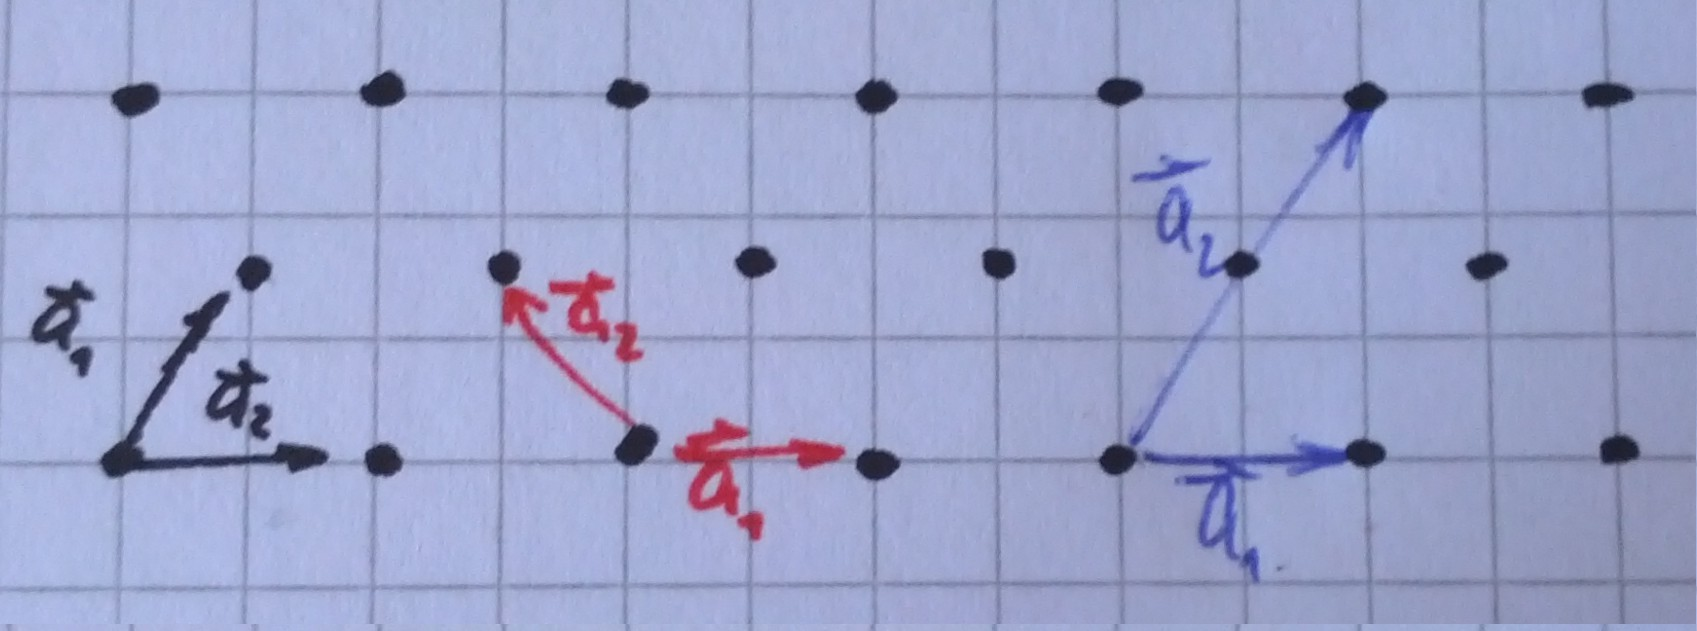
\includegraphics[width=0.8\textwidth]{pics/pic001.jpg}
				\caption{Vektoren im Kristallgitter}
				\end{figure}

			




\end{document}